\documentclass[a4paper]{scrartcl}

\usepackage{float}
\usepackage{tikz}
\usetikzlibrary{arrows,automata}
\usepackage{pgf}
\usepackage[utf8]{inputenc} % this is needed for umlauts
\usepackage[ngerman]{babel} % this is needed for umlauts
\usepackage[T1]{fontenc}    % this is needed for correct output of umlauts in pd
\usepackage{amssymb}
\usepackage{amsmath}
\usepackage{mathrsfs}
\usepackage{dsfont}
\usepackage{graphicx}
\usepackage{fancyhdr}
\usepackage{lastpage}
\usepackage{imakeidx}
\setlength{\parskip}{\medskipamount}
\setlength{\parindent}{0pt}
\usepackage{enumitem}
\usepackage{hyperref}
\usepackage{verbatim}

%%%%%%%%%%%%%%%%%%%%%%%%
% Kopf- und Fusszeilen %
%%%%%%%%%%%%%%%%%%%%%%%%
\pagestyle{fancy}
\lhead{
        Maximilian Roth
}
\chead{Logik-Tutorat Lösungen Blatt 5\\}
\rhead{
        \today{} \\
        Seite \thepage{} von \pageref{LastPage}\\
        
}
\lfoot{}
\cfoot{}
\rfoot{} 

%%%%%%%%%%%%%%%%%%%%%%%%
% Anfang des Dokuments %
%%%%%%%%%%%%%%%%%%%%%%%%

\begin{document}
\section*{Disclaimer}%{{{
\label{sec:disclaimer}
Auch in diesem Dokument können sich Fehler befinden!\\
Sie sind nicht die Musterlösung der Aufgaben, sondern selbst erstellte Lösungen.\\

Als generelle Lektüre kann ich nur das Skript von Markus Junker aus dem WS 17/18 empfehlen:\\
\url{http://home.mathematik.uni-freiburg.de/junker/skripte/InfoLogik.pdf}\\
Hier ist vieles sehr genau und verständlich erklärt.%}}}

\section*{}%{{{
\label{sec:aufgabe_1}

    \begin{figure}[H]
        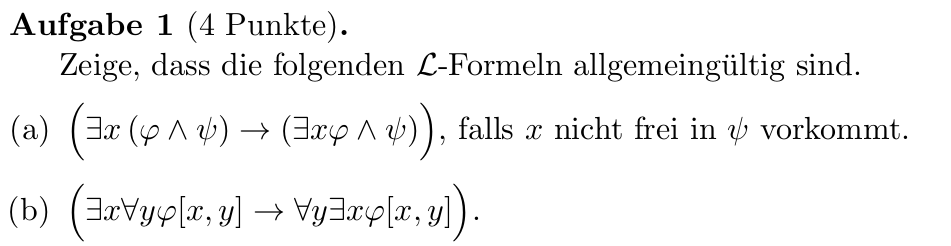
\includegraphics[scale=0.3]{./A-1.png}
        \label{fig:}
    \end{figure}

    \begin{itemize}
        \item a)\\
            Sei $\mathfrak{A}$ beliebige $\mathscr{L}$-Struktur.\\
            \\\underline{Annahme:} $\mathfrak{A} \nvdash (\exists x(\varphi \land \psi) \rightarrow (\exists x \varphi \land \psi))$\\
            $\Rightarrow$ es gibt eine Belegung $x_1,\dots,x_n: \mathfrak{A} \vdash \exists x(\varphi \land \psi)$, 
            aber $\mathfrak{A} \nvdash (\exists x \varphi \land \psi)$\\
            Aus $\mathfrak{A} \vdash \exists x (\varphi \land \psi)$ folgt aber: $\mathfrak{A} \vdash \exists x \varphi$ und $\mathfrak{A} \vdash \exists x \psi$\\
            $\overset{\text{x nicht frei in } \psi}{\Rightarrow} \mathfrak{A} \vdash \psi$\\
            $\Rightarrow \mathfrak{A} \vdash (\exists x \varphi \land \psi)$ Widerspruch! 
            Es gilt $\mathfrak{A} \vdash (\exists x(\varphi \land \psi) \rightarrow (\exists x \varphi \land \psi))$\\
        \item b)\\
            Sei $\mathfrak{A} \text{ beliebige } \mathscr{L}\text{-Struktur.}$\\
            \\Gilt $\mathfrak{A} \vdash \exists x \forall y \varphi[x,y]$, dann folgt:\\
            Es gibt ein $a \in A: \mathfrak{A} \vdash \forall y \varphi[a,y]$ d.h.:\\
            Für alle $b \in A$ gilt: $\mathfrak{A} \vdash \varphi[a,b]$\\
            $\Rightarrow \vdash \forall y \exists x \varphi[x,y]$ nämlich mindestens a
    \end{itemize}%}}}

\section*{}%{{{
\label{sec:aufgabe_2}

    \begin{figure}[H]
        \centering
        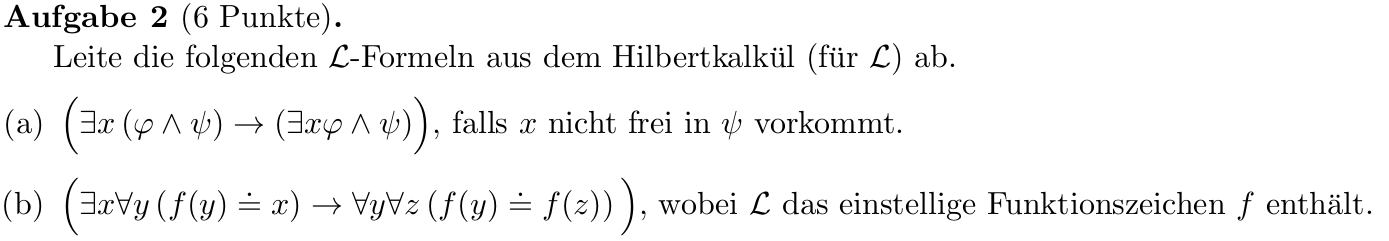
\includegraphics[scale=0.3]{./A-2.png}
        \label{fig:}
    \end{figure}

    \begin{figure}[H]
        \centering
        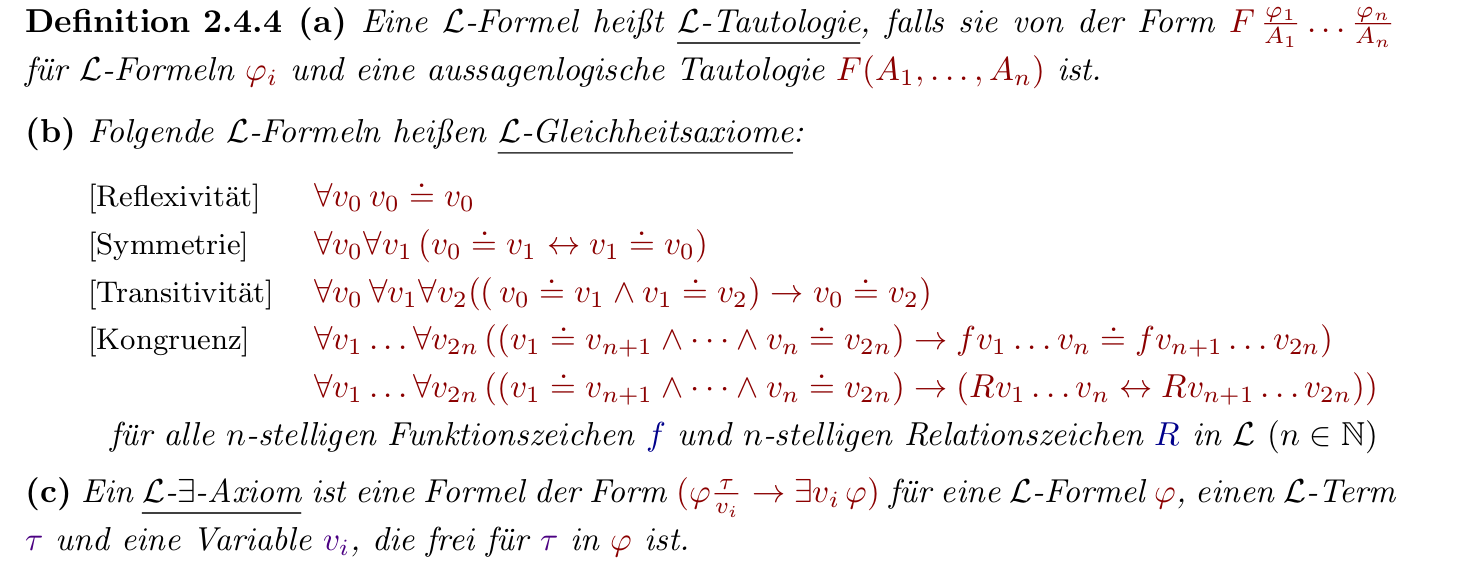
\includegraphics[scale=0.3]{./Allg.png}
        \label{fig:./Allg}
    \end{figure}

    \begin{figure}[H]
        \centering
        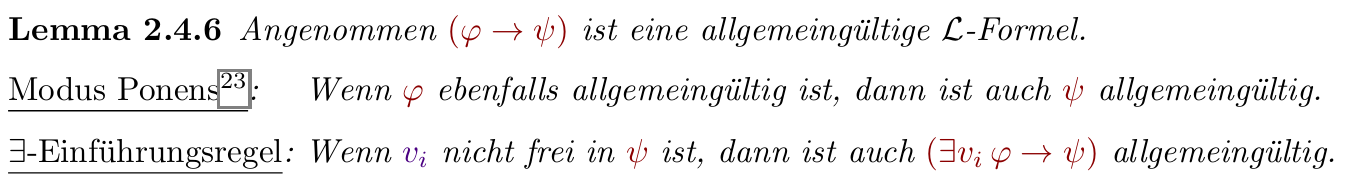
\includegraphics[scale=0.3]{./MP.png}
        \label{fig:./MP}
    \end{figure}

    \begin{itemize}
        \item a)\\
            \begin{itemize}
                \item Version 1:\\
                    Nach Definition enthält das Hilbert-Kalkül alle $\mathscr{L}$-Tautologien als Axiome.\\
                    $\overset{1 a)}{\Rightarrow} \vdash (\exists x(\varphi \land \psi) \rightarrow (\exists x \varphi \land \psi))$\\
                \item Version 2:\\
                    Nach $\exists$-Axiom: $\vdash (\varphi \rightarrow \exists x \varphi)$\\
                    Wir wissen auch: $\vdash ((\varphi \rightarrow \exists x \varphi) \rightarrow ((\varphi \land \psi) \rightarrow (\exists x \varphi \land \psi)))$\\
                    Wenden wir nun Modus Ponens ($\vdash (\varphi \rightarrow \psi)$ und $\vdash \varphi \Rightarrow \vdash \psi$) an\\
                    $\vdash ((\varphi \land \psi) \rightarrow (\exists x \varphi \land \psi))$\\
                    Und zuletzt mit der $\exists$-Einführungsregel (x ist nicht frei in $(\exists x \varphi \land \psi)$):\\
                    $\vdash (\exists x(\varphi \land \psi) \rightarrow (\exists x \varphi \land \psi))$\\
            \end{itemize}
        \item b)\\

    \end{itemize}%}}}

\section*{}%{{{
\label{sec:aufgabe_3}

    \begin{figure}[H]
        \centering
        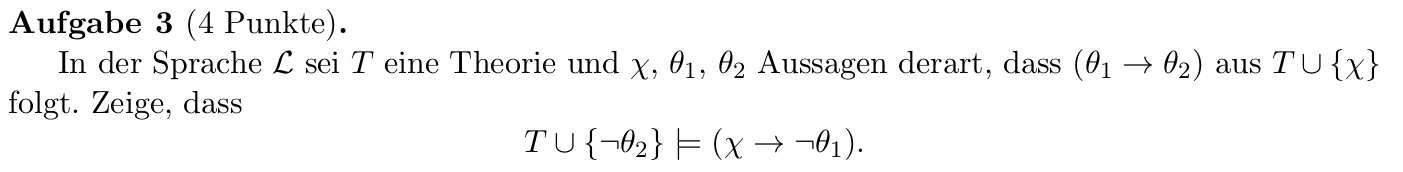
\includegraphics[scale=0.3]{./A-3.png}
        \label{fig:}
    \end{figure}

    \underline{Beweis:}\\
        Sei $\mathfrak{A} \vDash T \cup \{\neg \Theta_2\}$
        $\mathfrak{A} \vDash \chi\\
        \overset{Aufgabe}{\Rightarrow} \mathfrak{A} \vDash (\Theta_1 \rightarrow \Theta_2)\\
        \overset{\neg \Theta_2}{\Rightarrow} \mathfrak{A} \vDash \neg \Theta_1$\\
        $\Rightarrow \mathfrak{A} \vDash (\chi \rightarrow \Theta_1)$\\

%}}}

\section*{}%{{{
\label{sec:aufgabe_4}

    \begin{figure}[H]
        \centering
        
\includegraphics[scale=0.3]{./A-4.png}
        \label{fig:}
    \end{figure}

    \begin{itemize}
        \item a)\\
            \underline{Beweis:}\\
            \begin{itemize}
                \item Universum einer Unterstruktur von $ \mathfrak{M}$\\
                \\Da $\mathscr{L}$ weder Funktions- noch Konstantenzeichen hat ist jede Teilmenge von M auch Grundmenge einer Unterstruktur.\\
                Und da $F(\mathds{R}) \subseteq M \Rightarrow F(\mathds{R})$ ist Grundmenge einer Unterstruktur von $\mathfrak{M}$.\\
    \item $F(\mathcal{R}) \simeq \mathcal{R}$\\
                \\Achtung informell: Wir nehmen die 'vorhandene' Einbettung F und betrachten nur die Unterstruktur $F(\mathcal{R})$ als 'Ziel'. Da F inj. folgt die neue
                    Einbettung ist bij.\\
                \begin{itemize}
                    \item Wir zeigen zunächst, dass $F(\mathcal{R})$ Unterstruktur von $ \mathfrak{M}$ ist.\\
                        \begin{itemize}
                            \item Wir wissen bereits, dass $F(\mathcal{R}) \subseteq M$ ist.\\
                            \item Also bleibt noch, dass $Id_{F(\mathds{R})}: F(\mathds{R}) \rightarrow M$ Einbettung ist.\\
                                Dafür müssen wir zeigen, dass $Id_{F(\mathds{R})}$ mit < kompatibel ist,\\
                                dies wissen wir aber bereits, da F schon Einbettung war.\\
                        \end{itemize}
                        Daraus folgt, dass $F(\mathcal{R})$ Unterstruktur von $ \mathfrak{M}$ ist.\\
                    \item Nun ist die eingeschränkte Funktion\\
                        $G: \mathcal{R} \rightarrow F(\mathcal{R}), G: r \mapsto F(r)$ eine Einbettung von $\mathcal{R} \text{ in } F(\mathcal{R})$.\\
                    \item Da F injektiv war und $|\mathcal{R}| = |F(\mathcal{R})| \Rightarrow$ G bijektiv.\\
                \end{itemize}
                $\Rightarrow F(\mathcal{R}) \simeq \mathcal{R}$.\\
            \end{itemize}
       
\newpage

        \item b)\\
            \underline{ZZ:} $ \mathfrak{N} \vDash Diag^{at}(\mathcal{R}) \Leftrightarrow \text{ F Einbettung}$\\
            \\\underline{Beweis:}\\
            \begin{itemize}
                \item F Einbettung $\Rightarrow \mathcal{N} \vDash Diag^{at}(\mathcal{R})$\\
                    Sei $\varphi$ quantorenfreie $ \mathscr{L}(\mathds{R})$-Aussage\\
                    \\$\mathcal{N} \vDash \varphi\\
                    \overset{F(\mathcal{R}) \subset \mathcal{N}\text{ 4 b) Blatt 3}}{\Leftrightarrow} F(\mathcal{R}) \vDash \varphi\\
                    \overset{F(\mathcal{R}) \simeq \mathcal{R}}{\Leftrightarrow} \mathcal{R} \vDash \varphi\\
                    \overset{Aufgabe}{\Leftrightarrow} \varphi \in Diag^{at}(\mathcal{R})\\
                    \\\Rightarrow \mathcal{N} \vDash Diag^{at}(\mathcal{R})$\\

                \item $\mathcal{N} \vDash Diag^{at}(\mathcal{R}) \Rightarrow$ F Einbettung\\
                    \begin{itemize}
                        \item F ist offensichtlich injektiv.\\
                        \item Konstanten, Funktionen und Relationen sind kompatibel:\\
                            \begin{itemize}
                                \item Konstanten:\\
                                    $F(d_r^{\mathcal{R}}) = F(r) = F(d_r^{\mathcal{N}})$\\
                                \item Funktionen: Nicht vorhanden\\
                                \item Relationen:\\
                                    $(s,t) \in <^\mathcal{R} \Leftrightarrow d_s < d_t \in Diag^{at}(\mathcal{R})\\
                                    \Leftrightarrow \mathcal{N} \vDash d_s < d_t
                                    \Leftrightarrow (d_s,d_t) \in <^\mathcal{N} \Leftrightarrow (F(s),F(t)) \in <^\mathcal{N}$\\
                                    \\Wir haben gekonnt $(s,t)$, was keine quantorenfreie $\mathscr{L}(\mathcal{R})$-Aussage ist zu $d_s < d_t$, 
                                    was eine solche ist überführt.\\
                                    Dann haben wir nur noch die Annahme genutzt.\\
                            \end{itemize}
                    \end{itemize} 
                    $\Rightarrow$ F ist Einbettung
            \end{itemize}

            \begin{figure}[H]
                \centering
                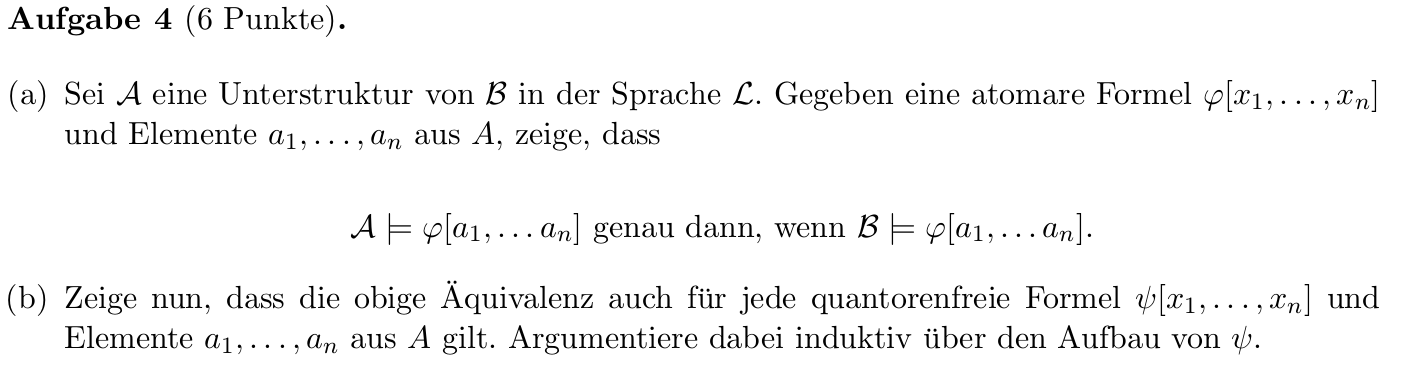
\includegraphics[scale=0.3]{./B3-4-b.png}
                \caption{Von Blatt 3}
                \label{fig:./B3-4-b}
            \end{figure}
        
        \item c)\\
            Diag$(\mathcal{R}) = \{\varphi \mathscr{L}-Auss | \mathcal{R} \vDash \varphi\}$\\
            \\\underline{ZZ:} 
            Wenn $\mathcal{N} \mathscr{L}(\mathds{R})$-Struktur: $\mathcal{N} \vDash Diag(\mathcal{R}) \Leftrightarrow F(\mathcal{R}) \preceq \mathcal{N}$\\
            \\\underline{Beweis:}\\

            \begin{itemize}
                \item $\mathcal{N} \vDash Diag(\mathcal{R}) \Rightarrow F(\mathcal{R}) \preceq \mathcal{N}$\\
                    Aus a) wissen wir, dass  $F(\mathcal{R}) \subset \mathcal{N}$, aus  b), dass F Einbettung ist.\\
                    \\Sei $\varphi \text{  } \mathscr{L}(\mathds{R})$-Formel\\
                    \begin{equation*}
                        \begin{split}
                            \label{eq:}
                            & F(\mathcal{R} \vDash \varphi[r_1,\dots,r_n])\\
                            \Rightarrow & F(\mathcal{R} \vDash \varphi[r_1^{F(\mathcal{R})},\dots,r_n^{\mathcal{R}}])\\
                            \overset{\text{R als }\mathscr{L}(\mathcal{R}) \text{-Struktur } \simeq F(\mathcal{R})}{\Rightarrow} & \mathcal{R} \vDash
                            \varphi[d_{r_1}^\mathcal{R},\dots,d_{r_n}^\mathcal{R}]\\
                            \overset{Aufgabe}{\Rightarrow} & \varphi[d_{r_1}^\mathcal{R},\dots,d_{r_n}^\mathcal{R}] \in Diag(\mathcal{R})\\
                            \Rightarrow & \mathcal{N} \vDash \varphi[d_{r_1}^{F(\mathcal{R})},\dots,d_{r_n}^{F(\mathcal{R})}]\\
                            \Rightarrow & \mathcal{N} \vDash \varphi[r_1,\dots,r_n]\\
                        \end{split}
                    \end{equation*}
                    \\Da dies für alle $\varphi$ gilt folgt: $F(\mathcal{R}) \preceq \mathcal{N}$\\
            
                \item $F(\mathcal{R} \preceq \mathcal{N}) \Rightarrow \mathcal{N} \vDash Diag(\mathcal{R})$\\
                    \\Sei $\varphi \in Diag(\mathcal{R}) \text{, also } \mathscr{L}$- Aussage.\\
                    $\overset{Aufgabe}{\Leftrightarrow} \mathcal{R} \vDash \varphi$\\
                    $\overset{\mathcal{R} \simeq F(\mathcal{R})}{\Leftrightarrow} F(R) \vDash \varphi$\\
                    $\overset{F(\mathcal{R}) \preceq \mathcal{N}}{\Leftrightarrow}\mathcal{N} \vDash \varphi$\\
                    \\$\mathcal{N} \vDash Diag(\mathcal{R})$\\


            \end{itemize}

            \begin{figure}[H]
                \centering
                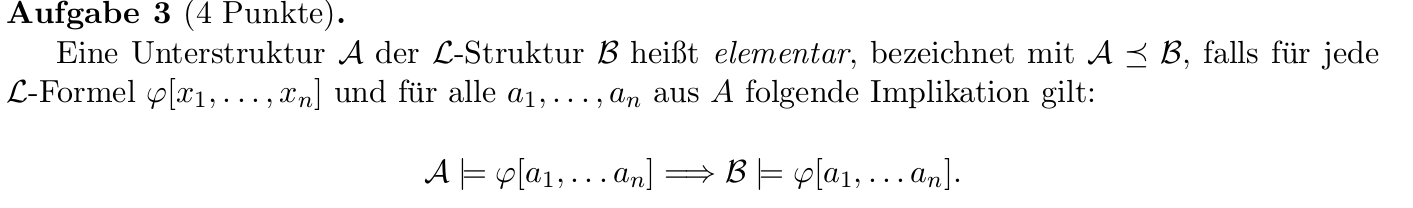
\includegraphics[scale=0.3]{./B4-3.png}
                \caption{Von Blatt 4}
                \label{fig:./B4-3}
            \end{figure}
            


    \end{itemize}

%}}}
\end{document}
